%!Tex Root = ../Main.tex
% ./Packete_und_Deklarationen.tex
% ./Titlepage.tex
% ./Motivation.tex
% ./Einführung.tex
% ./Implementierung2.tex
% ./Ergebnisse_und_Ausblick.tex

\chapter{Implementierung}
\label{ch:implementierung}

\section{Lexikalische Analyse}
\subsection{Konkrette Syntax für Lexer erstellen}
\numberwithin{floatgrammar}{section}

\label{sec:lex_analyse_verwendung_von_lark}
% ./concrete_syntax_picoc.lark
\begin{grammar}[Konkrette Syntax des Lexers in EBNF][H][gr:concrete_syntax_lex]
  \toprule
  \firstcase{COMMENT}{\dq //\dq\enspace /[{\wedge}\backslash n]{*}/\gralt \dq {/*}\dq\enspace  /(.\mid \setminus n)*?/\enspace \dq {*/}\dq }{L\_Comment}
  \firstcase{RETI\_COMMENT.2}{\dq {//}\dq \dq \text{\textvisiblespace} \dq ? \dq \#\dq /[\wedge\backslash n]{*}/}{}
  \midrule
  \firstcase{DIG\_NO\_0}{\dq 1\dq \gralt \dq 2\dq \gralt \dq 3\dq \gralt \dq 4\dq \gralt \dq 5\dq}{L\_Arith}
  \otherform{\dq 6\dq \gralt \dq 7\dq \gralt \dq 8\dq \gralt \dq 9\dq}{}
  \firstcase{DIG\_WITH\_0}{\dq 0\dq \gralt DIG\_NO\_0}{}
  \firstcase{NUM}{\dq 0\dq \gralt DIG\_NO\_0 DIG\_WITH\_0*}{}
  \firstcase{ASCII\_CHAR}{\dq\text{\textvisiblespace} \dq ..\dq \sim\dq }{}
  \firstcase{CHAR}{\dq '\dq ASCII\_CHAR\dq '\dq }{}
  \firstcase{FILENAME}{ASCII\_CHAR+\dq .picoc\dq }{}
  \firstcase{LETTER}{\dq {a}\dq ..\dq {z}\dq \gralt \dq {A}\dq ..\dq {Z}\dq}{}
  \firstcase{NAME}{(LETTER\gralt \dq \_\dq )}{}
  & & \qquad(LETTER\gralt DIG\_WITH\_0\gralt \dq \_\dq )* & \\
  \firstcase{name}{NAME\gralt INT\_NAME\gralt CHAR\_NAME}{}
  \otherform{VOID\_NAME}{}
  \firstcase{NOT}{\dq \sim\dq }{}
  \firstcase{REF\_AND}{\dq \&\dq }{}
  \firstcase{un\_op}{SUB\_MINUS\gralt LOGIC\_NOT\gralt NOT}{}
  \otherform{MUL\_DEREF\_PNTR \gralt REF\_AND}{}
  \firstcase{MUL\_DEREF\_PNTR}{\dq {*}\dq }{}
  \firstcase{DIV}{\dq /\dq }{}
  \firstcase{MOD}{\dq \%\dq }{}
  \firstcase{prec1\_op}{MUL\_DEREF\_PNTR\gralt DIV\gralt MOD}{}
  \firstcase{ADD}{\dq {+}\dq }{}
  \firstcase{SUB\_MINUS}{\dq {-}\dq }{}
  \firstcase{prec2\_op}{ADD\gralt SUB\_MINUS}{}
  \midrule
  \firstcase{LT}{\dq {<}\dq }{L\_Logic}
  \firstcase{LTE}{\dq {<=}\dq }{}
  \firstcase{GT}{\dq {>}\dq }{}
  \firstcase{GTE}{\dq {>=}\dq }{}
  \firstcase{rel\_op}{LT\gralt LTE\gralt GT\gralt GTE}{}
  \firstcase{EQ}{\dq {==}\dq }{}
  \firstcase{NEQ}{\dq {!=}\dq }{}
  \firstcase{eq\_op}{EQ\gralt NEQ}{}
  \firstcase{LOGIC\_NOT}{\dq !\dq }{}
  \midrule
  \firstcase{INT\_DT.2}{\dq int\dq }{}
  \firstcase{INT\_NAME.3}{\dq int\dq\enspace (LETTER\gralt DIG\_WITH\_0\gralt \dq \_\dq )+}{L\_Assign\_Alloc}
  \firstcase{CHAR\_DT.2}{\dq char\dq }{}
  \firstcase{CHAR\_NAME.3}{\dq char\dq\enspace (LETTER\gralt DIG\_WITH\_0\gralt \dq \_\dq )+}{}
  \firstcase{VOID\_DT.2}{\dq void\dq }{}
  \firstcase{VOID\_NAME.3}{\dq void\dq\enspace (LETTER\gralt DIG\_WITH\_0\gralt \dq \_\dq )+}{}
  \firstcase{prim\_dt}{INT\_DT\gralt CHAR\_DT\gralt VOID\_DT}{}
  \bottomrule
\end{grammar}

% \begin{grammar}[\(\lambda\) calculus syntax][p][gr:ex1]
%   \firstcase{T}{\nonterm{V}}{Variable}
%   \otherform{(\nonterm{T}\ \nonterm{T})}{Application}
%   \otherform{\lambda \nonterm{V}\cdot\nonterm{T}}{Abstraction}
%   \firstcase{V}{x, y, \dots}{Variables}
% \end{grammar}
% \begin{grammar}[Advanced capabilities of \texttt{grammar.sty}][p][gr:ex2]
%   \firstcase{A}{\nonterm{T} \gralt \nonterm{V}}{Multiple option on a single line}
%   \highlight
%   \otherform{\nonterm{A}}{Highlighted form}
%   \downplay
%   \otherform{\nonterm{B}\gralt \nonterm{C}}{Downplayed form}
%   \otherform{\lochighlight{\nonterm{A}} \gralt \nonterm{B}}{Emphasize part of the line}
% \end{grammar}

% erwähnen, dass in Lark die Grammatiken L_Lex und L_Parse gemischt sind
% EBNF erwähnen
% (erwähnen, dass finalle Grammatik im Appendix)
\subsection{Basic Lexer}
\section{Syntaktische Analyse}
\subsection{Konkrette Syntax für Parser erstellen}
% ./concrete_syntax_picoc.lark
% https://tex.stackexchange.com/questions/851/removing-spaces-between-words-in-math-mode
In \ref{gr:concrete_syntax_parser}

\begin{grammar}[Konkrette Syntax des Parsers in EBNF, Teil 1][H][gr:concrete_syntax_parser]
  \toprule
	\downplay
  \firstcase{prim\_exp}{name\gralt NUM\gralt CHAR\gralt "("logic\_or")"}{L\_Arith +}
	\downplay
  \firstcase{post\_exp}{array\_subscr\gralt struct\_attr\gralt fun\_call}{L\_Array +}
	\downplay
  \otherform{input\_exp\gralt print\_exp\gralt prim\_exp}{L\_Pntr +}
	\downplay
  \firstcase{un\_exp}{un\_op un\_exp\gralt post\_exp}{L\_Struct + L\_Fun}
  \midrule
	\downplay
  \firstcase{input\_exp}{\dq input\dq\dq(\dq\dq)\dq}{L\_Arith}
	\downplay
  \firstcase{print\_exp}{\dq print\dq\dq(\dq logic\_or\dq)\dq}{}
	\downplay
  \firstcase{arith\_prec1}{arith\_prec1\enspace prec1\_op\enspace un\_exp\gralt un\_exp}{}
	\downplay
  \firstcase{arith\_prec2}{arith\_prec2\enspace prec2\_op\enspace arith\_prec1\gralt arith\_prec1}{}
	\downplay
  \firstcase{arith\_and}{arith\_and\enspace \dq\&\dq\enspace arith\_prec2\gralt arith\_prec2}{}
	\downplay
  \firstcase{arith\_oplus}{arith\_oplus\enspace \dq {\wedge{}}\dq\enspace arith\_and\gralt arith\_and}{}
	\downplay
  \firstcase{arith\_or}{arith\_or\enspace \dq{\mid} \dq\enspace arith\_oplus\gralt arith\_oplus}{}
  \midrule
  \downplay
  \firstcase{rel\_exp}{rel\_exp\enspace rel\_op\enspace arith\_or\gralt arith\_or}{L\_Logic}
  \downplay
  \firstcase{eq\_exp}{eq\_exp\enspace eq\_op rel\_exp\gralt rel\_exp}{}
  \downplay
  \firstcase{logic\_and}{logic\_and\enspace \dq{\&\&}\dq\enspace eq\_exp\gralt eq\_exp}{}
  \downplay
  \firstcase{logic\_or}{logic\_or\enspace \dq{\mid\mid}\dq\enspace logic\_and\gralt logic\_and}{}
  \midrule
	\downplay
  \firstcase{type\_spec}{prim\_dt\gralt struct\_spec}{L\_Assign\_Alloc}
	\downplay
  \firstcase{alloc}{type\_spec\enspace pntr\_decl}{}
	\downplay
  \firstcase{assign\_stmt}{un\_exp\enspace \dq {=}\dq\enspace logic\_or\dq ;\dq }{}
  \firstcase{initializer}{logic\_or\gralt array\_init\gralt struct\_init}{}
	\downplay
  \firstcase{init\_stmt}{alloc\enspace \dq {=}\dq\enspace initializer\dq ;\dq }{}
	\downplay
  \firstcase{const\_init\_stmt}{\dq const\dq\enspace type\_spec\enspace name\enspace \dq {=}\dq\enspace NUM\dq ;\dq }{}
  \midrule
  \firstcase{pntr\_deg}{\dq {*}\dq *}{L\_Pntr}
  \firstcase{pntr\_decl}{pntr\_deg\enspace array\_decl\gralt array\_decl}{}
  \midrule
  \firstcase{array\_dims}{(\dq [\dq NUM\dq ]\dq )*}{L\_Array}
  \firstcase{array\_decl}{name\enspace array\_dims\gralt \dq (\dq pntr\_decl\dq )\dq  array\_dims}{}
  \firstcase{array\_init}{\dq \{\dq initializer(\dq ,\dq\enspace initializer)*\dq \}\dq }{}
  \firstcase{array\_subscr}{post\_exp\dq [\dq logic\_or\dq ]\dq }{}
  \midrule
  \firstcase{struct\_spec}{\dq struct\dq\enspace name}{L\_Struct}
  \firstcase{struct\_params}{(alloc\dq ;\dq )+}{}
  \firstcase{struct\_decl}{\dq struct\dq\enspace name\enspace \dq \{\dq struct\_params\dq \}\dq }{}
  \firstcase{struct\_init}{\dq \{\dq \dq .\dq name\dq {=}\dq initializer}{}
  & & \qquad(\dq ,\dq\enspace \dq .\dq name\dq {=}\dq initializer)*\dq \}\dq & \\
  \firstcase{struct\_attr}{post\_exp\dq .\dq name}{}
  \midrule
	\downplay
  \firstcase{if\_stmt}{\dq if\dq \dq (\dq logic\_or\dq )\dq\enspace exec\_part}{L\_If\_Else}
	\downplay
  \firstcase{if\_else\_stmt}{\dq if\dq \dq (\dq logic\_or\dq )\dq\enspace exec\_part\enspace \dq else\dq\enspace exec\_part}{}
  \midrule
	\downplay
  \firstcase{while\_stmt}{\dq while\dq \dq (\dq logic\_or\dq )\dq\enspace exec\_part}{L\_Loop}
	\downplay
  \firstcase{do\_while\_stmt}{\dq do\dq\enspace exec\_part\enspace \dq while \dq \dq (\dq logic\_or\dq )\dq \dq ;\dq }{}
  \bottomrule
\end{grammar}

\begin{grammar}[Konkrette Syntax des Parsers in EBNF, Teil 2][H]
  \toprule
	\downplay
  \firstcase{decl\_exp\_stmt}{alloc\dq ;\dq }{L\_Stmt}
	\downplay
  \firstcase{decl\_direct\_stmt}{ assign\_stmt\gralt init\_stmt\gralt const\_init\_stmt}{}
  \firstcase{decl\_part}{ decl\_exp\_stmt\gralt decl\_direct\_stmt\gralt RETI\_COMMENT}{}
  \\[-0.2cm]
	\downplay
  \firstcase{compound\_stmt}{ \dq \{\dq exec\_part* \dq \}\dq }{}
	\downplay
  \firstcase{exec\_exp\_stmt}{logic\_or\dq ;\dq }{}
	\downplay
  \firstcase{exec\_direct\_stmt}{if\_stmt\gralt if\_else\_stmt\gralt while\_stmt\gralt do\_while\_stmt}{}
	\downplay
  \otherform{assign\_stmt\gralt fun\_return\_stmt}{}
  \firstcase{exec\_part}{compound\_stmt\gralt exec\_exp\_stmt\gralt exec\_direct\_stmt}{}
  \otherform{RETI\_COMMENT}{}
  \\[-0.2cm]
  \firstcase{decl\_exec\_stmts}{decl\_part* exec\_part*}{}
  \midrule
  \firstcase{fun\_args}{[logic\_or(\dq ,\dq\enspace logic\_or)*]}{L\_Fun}
  \firstcase{fun\_call}{name\dq (\dq fun\_args\dq )\dq }{}
  \firstcase{fun\_return\_stmt}{\dq return\dq\enspace [logic\_or]\dq ;\dq }{}
  \firstcase{fun\_params}{[alloc(\dq ,\dq\enspace alloc)*]}{}
  \firstcase{fun\_decl}{type\_spec\enspace pntr\_deg\enspace name\dq (\dq fun\_params\dq )\dq }{}
  \firstcase{fun\_def}{type\_spec\enspace pntr\_deg\enspace name\dq (\dq fun\_params\dq )\dq\enspace \dq \{\dq  decl\_exec\_stmts \dq \}\dq }{}
  \midrule
  \firstcase{decl\_def}{(struct\_decl\gralt fun\_decl)\dq ;\dq \gralt fun\_def}{L\_File}
  \firstcase{decls\_defs}{decl\_def*}{}
  \firstcase{file}{FILENAME\enspace decls\_defs}{}
  \bottomrule
\end{grammar}
% Vorteile von Lark
\subsection{Umsetzung von Präzidenz}
Die \colorbold{PicoC} Programmiersprache hat dieselben \colorbold{Präzidenzregeln} implementiert, wie die Programmiersprache \colorbold{C} \footcite{noauthor_c_nodate}. Die \colorbold{Präzidenzregeln} von \colorbold{PicoC} sind in Tabelle~\ref{tab:reference_table} aufgelistet.

% \rowcolors{2}{SecondaryColor}{white}
\begin{table}[H]
  \center
  % \Block{2}{=}{Links, dann rechts $\rightarrow$} \\
  \begin{NiceTabular}{X[1,c]X[2,c]X[3,l]X[2,c]}[rules/color=PrimaryColor] % {\linewidth}{|C|C|L|L|}
  \CodeBefore
  \rowcolor{PrimaryColor}{1}
  \rowcolors{2-18}{SecondaryColor}{}[cols={1-3}]
  \rowcolors{2-18}{SecondaryColor}{}[cols={4}, respect-blocks, restart]
  \Body
  \textbf{\textcolor{white}{Präzidenz}} &	\textbf{\textcolor{white}{Operator}} & \textbf{\textcolor{white}{Beschreibung}} &	\textbf{\textcolor{white}{Assoziativität}} \\
  1	& \verb|a()|	& Funktionsaufruf & \Block{3-1}{Links, dann rechts $\rightarrow$} \\
    & \verb|a[]|	& Indexzugriff & \\
    & \verb|a.b| & Attributzugriff & \\
  2	&	\verb|-a| & Unäres Minus & \Block{3-1}{Rechts, dann links $\leftarrow$} \\
    & \smalltt{!a $\thicksim$a}	& Logisches NOT und Bitweise NOT & \\
    & \verb|*a &a| & Dereferenz und Referenz, auch Adresse-von & \\
  3	& \smalltt{a*b a/b a\%b} &	Multiplikation, Division und Modulo & \Block{9-1}{Links, dann rechts $\rightarrow$} \\
  4	& \verb|a+b a-b|	& Addition und Subtraktion & \\
  5	& \verb|a<b a<=b| \verb|a>b a>=b| & Kleiner, Kleiner Gleich, Größer, Größer gleich & \\
  6 &	\verb|a==b a!=b| & Gleichheit und Ungleichheit & \\
  7 &	\verb|a&b| & Bitweise UND & \\
  8 &	\verb|a^b| & Bitweise XOR (exclusive or) & \\
  9 & \smalltt{a$\mid$b} & Bitweise ODER (inclusive or) & \\
  10	& \verb|a&&b| &	Logiches UND & \\
  11	& $a{\mid\mid} b$	& Logisches ODER & \\
  12 & \verb|a=b| & Zuweisung & Rechts, dann links $\leftarrow$ \\
  13 &	\verb|a,b|& Komma	& Links, dann rechts $\rightarrow$ \\
  \bottomrule
\end{NiceTabular}
\caption{Präzidenzregeln von PicoC}
\label{tab:reference_table}
\end{table}
% erwähnen von Mehrdeutigkeit und Assoziativität
% finalle Grammatik im Appendix
% Crafting Compilers Quelle benennen

\subsection{Derivation Tree Generierung}
\subsubsection{Early Parser}
\subsubsection{Codebeispiel}
\label{sec:derivation_tree_generierung}
\begin{code}
  \centering
  \numberedcodebox[minted language=c]{./code_examples/example_dt_simple_ast_gen_array_decl_and_alloc.picoc}
  \caption{PicoC Code für Derivation Tree Generierung}
  \label{code:picoc_code_für_derivation_tree_generierung}
\end{code}

\begin{code}
  \centering
  \numberedcodebox[minted language=text]{./code_examples/example_dt_simple_ast_gen_array_decl_and_alloc.dt}
  \caption{Derivation Tree nach Derivation Tree Generierung}
  \label{code:derivation_tree_nach_derivation_tree_generierung}
\end{code}

\subsection{Derivation Tree Vereinfachung}
\subsubsection{Visitor}
\subsubsection{Codebeispiel}

Beispiel aus Subkapitel~\ref{sec:derivation_tree_generierung} wird fortgeführt.

\begin{code}
  \centering
  \numberedcodebox[minted language=text]{./code_examples/example_dt_simple_ast_gen_array_decl_and_alloc.dt_simple}
  \caption{Derivation Tree nach Derivation Tree Vereinfachung}
  \label{code:picoc_code_nach_derivation_tree_vereinfachung}
\end{code}

% Visitor erwähnen
\subsection{Abstrakt Syntax Tree Generierung}
\subsubsection{PicoC Nodes}
% Tabelle aller PicoC Nodes
% möglichst kurze und leicht verständliche Bezeichner für Nodes
\subsubsection{RETI Nodes}
% Tabelle aller RETI Nodes
% Transformer erwähnen
\subsubsection{Abstrakte Syntax}

% ./abstract_syntax.txt
\newpage
\begin{grammar}[Abstrakte Syntax für $L_{PiocC}$][H][gr:abstract_syntax_l_picoc]
  \toprule
  \firstcase{un\_op}{Minus() \gralt Not()}{L\_Arith}
  \firstcase{bin\_op}{Add() \gralt Sub() \gralt Mul() \gralt Div() \gralt Mod()}{}
  \otherform{Oplus() \gralt And() \gralt Or()}{}
  \firstcase{exp}{Name(str) \gralt Num(str) \gralt Char(str)}{}
  \otherform{BinOp(\langle exp\rangle , \langle bin\_op\rangle , \langle exp\rangle )}{}
  \otherform{UnOp(\langle un\_op\rangle , \langle exp\rangle ) \gralt Call(Name('input'), None)}{}
  \firstcase{exp\_stmts}{Alloc(\langle type\_qual\rangle , \langle dataype\rangle , Name(str))}{}
  \otherform{Call(Name('print'), \langle exp\rangle )}{}
  \midrule
  \firstcase{un\_op}{LogicNot()}{L\_Logic}
  \firstcase{rel}{Eq() \gralt NEq() \gralt Lt() \gralt LtE() \gralt Gt() \gralt GtE()}{}
  \firstcase{bin\_op}{LogicAnd() \gralt LogicOr()}{}
  \firstcase{exp}{Atom(\langle exp\rangle , \langle rel\rangle , \langle exp\rangle )}{}
  \otherform{ToBool(\langle exp\rangle )}{}
  \midrule
  \firstcase{type\_qual}{Const() \gralt Writeable()}{L\_Assign\_Alloc}
  \firstcase{datatype}{IntType() \gralt CharType() \gralt VoidType()}{}
  \firstcase{assign\_lhs}{Alloc(\langle type\_qual\rangle , \langle dataype\rangle , Name(str)) \gralt \langle rel\_loc\rangle }{}
  \firstcase{exp\_stmts}{Alloc(\langle type\_qual\rangle , \langle dataype\rangle , Name(str))}{}
  \firstcase{stmt}{Assign(\langle assign\_lhs\rangle , \langle exp\rangle )}{}
  \otherform{Exp(\langle exp\_stmts\rangle )}{}
  \midrule
  \firstcase{datatype}{PntrDecl(Num(str), \langle datatype\rangle )}{L\_Pntr}
  \firstcase{deref\_loc}{Ref(\langle ref\_loc\rangle )\gralt\langle ref\_loc\rangle }{}
  \firstcase{ref\_loc}{Name(str)}{}
  \otherform{Deref(\langle deref\_loc\rangle , \langle exp\rangle )}{}
  \otherform{Subscr(\langle deref\_loc\rangle , \langle exp\rangle )}{}
  \otherform{Attr(\langle ref\_loc\rangle , Name(str))}{}
  \firstcase{exp}{Deref(\langle deref\_loc\rangle , \langle exp\rangle )}{}
  \otherform{Ref(\langle ref\_loc\rangle )}{}
  \midrule
  \firstcase{datatype}{ArrayDecl(Num(str)+, \langle datatype\rangle )}{L\_Array}
  \firstcase{exp}{Subscr(\langle deref\_loc\rangle , \langle exp\rangle ) \gralt Array(\langle exp\rangle +)}{}
  \midrule
  \firstcase{datatype}{StructSpec(Name(str))}{L\_Struct}
  \firstcase{exp}{Attr(\langle ref\_loc\rangle , Name(str))}{}
  \otherform{Struct(Assign(Name(str), \langle exp\rangle )+)}{}
  \firstcase{decl\_def}{StructDecl(Name(str),}{}
  & & \qquad $Alloc(Writeable(), \langle datatype\rangle , Name(str))+)$ & \\
  \midrule
  \firstcase{stmt}{If(\langle exp\rangle , \langle stmt\rangle *)}{L\_If\_Else}
  \otherform{IfElse(\langle exp\rangle , \langle stmt\rangle *, \langle stmt\rangle *)}{}
  \midrule
  \firstcase{stmt}{While(\langle exp\rangle , \langle stmt\rangle *)}{L\_Loop}
  \otherform{DoWhile(\langle exp\rangle , \langle stmt\rangle *)}{}
  \midrule
  \firstcase{exp}{Call(Name(str), \langle exp\rangle *)}{L\_Fun}
  \firstcase{exp\_stmts}{Call(Name(str), \langle exp\rangle *)}{}
  \firstcase{stmt}{Return(\langle exp\rangle )}{}
  \firstcase{decl\_def}{FunDecl(\langle datatype\rangle , Name(str),}{}
  & & \qquad $Alloc(Writeable(), \langle datatype\rangle , Name(str))*)$ & \\
  \otherform{FunDef(\langle datatype\rangle , Name(str),}{}
  & & \qquad $Alloc(Writeable(), \langle datatype\rangle , Name(str))*, \langle stmt\rangle *)$ & \\
  \midrule
  \firstcase{file}{File(Name(str), \langle decl\_def\rangle *)}{L\_File}
  \bottomrule
\end{grammar}

% $L_{X}$ ist nicht notwendig sich zu überlegen, hier so getann als gäbe es diese Sprache
% Abstrakte Syntax ist für den Programmierer als Orientierungshilfe bei der Implementierung

\subsubsection{Transformer}

\subsubsection{Codebeispiel}
Beispiel welches in Subkapitel~\ref{sec:derivation_tree_generierung} angefangen wurde, wird hier fortgeführt.
% Transformer erwähnen, viel zu viel um es hier reinzumachen

\begin{code}
  \centering
  \numberedcodebox[minted language=text]{./code_examples/example_dt_simple_ast_gen_array_decl_and_alloc.ast}
  \caption{Abstract Syntax Tree aus vereinfachtem Derivarion Tree generiert}
  \label{code:abstract_syntax_tree_aus_vereinfachtem_derivarion_tree_generiert}
\end{code}

\section{Code Generierung}
\subsection{Übersicht}
% Unterscheid zur Architektur aus dem Bachelorprojekt

% Cross Compiler
% https://tex.stackexchange.com/questions/8625/force-figure-placement-in-text
\begin{figure}[H]
  \centering
  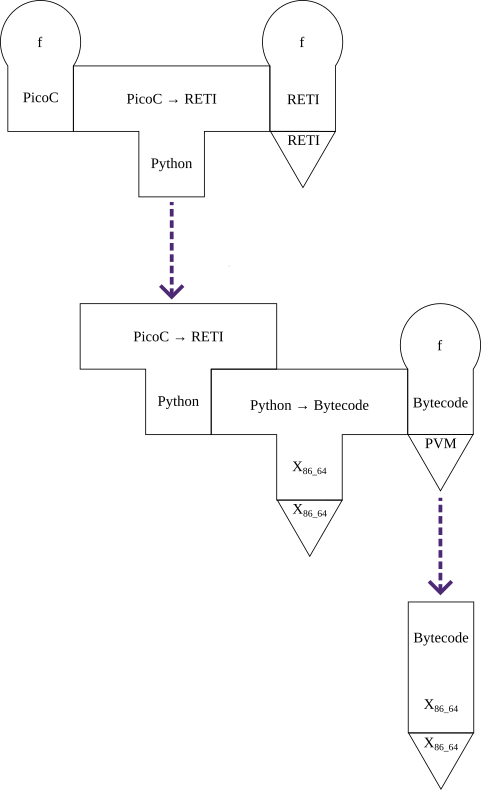
\includegraphics[width=0.5\linewidth]{./figures/summarized_cross_compiler.png}
  \caption{Cross-Compiler Kompiliervorgang ausgeschrieben}
\end{figure}

\begin{figure}[H]
  \centering
  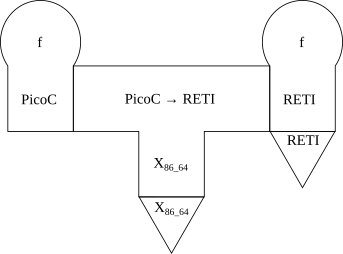
\includegraphics[width=0.33\linewidth]{./figures/compiliervorang_mit_machiene.png}
  \caption{Cross-Compiler Kompiliervorgang Kurzform}
\end{figure}

\begin{figure}[H]
  \centering
  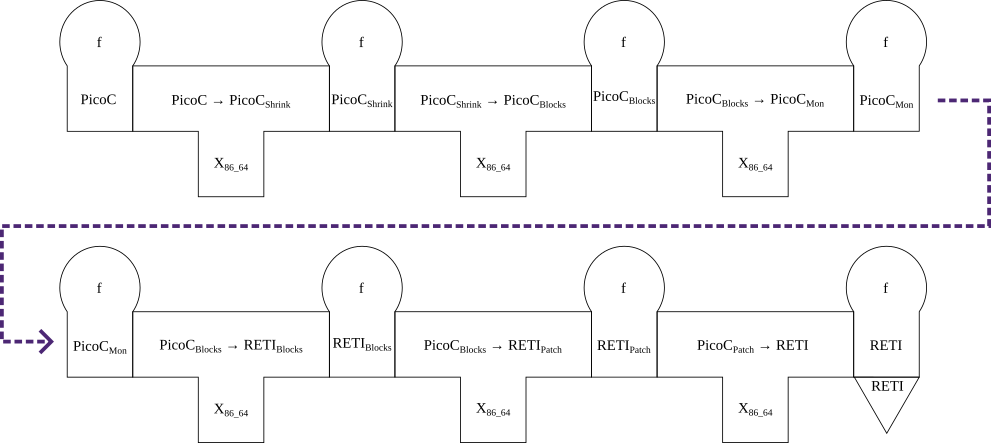
\includegraphics[width=\linewidth]{./figures/passes.png}
  \caption{Architektur mit allen Passes ausgeschrieben}
\end{figure}
\subsection{Passes}
\subsubsection{Kompositionen mit besonderer Bedeutung}
\subsubsection{PicoC-Shrink Pass}
\label{picoc_shrink_pass}
% dieser Pass existiert nur wegen der Erweiterungen

\newlineparagraph{Codebeispiel}

\begin{code}
  \centering
  \numberedcodebox[minted language=c]{./code_examples/example_faculty_it.picoc}
  \caption{PicoC Code für Codebespiel}
  \label{code:picoc_code_für_codebeispiel}
\end{code}

\begin{code}
  \centering
  \numberedcodebox[minted language=text]{./code_examples/example_faculty_it.ast}
  \caption{Abstract Syntax Tree für Codebespiel}
  \label{code:abstract_syntax_tree_für_codebeispiel}
\end{code}

\begin{code}
  \centering
  \numberedcodebox[minted language=text]{./code_examples/example_faculty_it.picoc_shrink}
  \caption{PicoC Shrink Pass für Codebespiel}
  \label{code:picoc_shrink_pass_für_codebeispiel}
\end{code}

\subsubsection{PicoC-Blocks Pass}
\newlineparagraph{Abstrakte Syntax}
\begin{grammar}[Abstrakte Syntax für $L_{PicoC\_Blocks}$][H][gr:abstract_syntax_l_picoc_blocks]
  \toprule
  \firstcase{decl\_def}{FunDef(\langle datatype\rangle , Name(str),}{L\_Fun}
  & & \qquad $Alloc(Writeable(), \langle datatype\rangle , Name(str))*, \langle block\rangle *)$ & \\
  \midrule
  \firstcase{block}{Block(Name(str), \langle stmt\rangle *)}{L\_Blocks}
  \firstcase{stmt}{Goto(Name(str)) \gralt NewStackframe(Name(), Goto(str))}{}
  \otherform{RemoveStackframe() \gralt SetScope(Name(str))}{}
  \otherform{SingleLineComment(str, str)}{}
  \bottomrule
\end{grammar}

\newlineparagraph{Codebeispiel}

\begin{code}
  \centering
  \numberedcodebox[minted language=text]{./code_examples/example_faculty_it.picoc_blocks}
  \caption{PicoC-Blocks Pass für Codebespiel}
  \label{code:picoc_blocks_pass_für_codebeispiel}
\end{code}

\subsubsection{PicoC-Mon Pass}
\newlineparagraph{Abstrakte Syntax}
\begin{grammar}[Abstrakte Syntax für $L_{PicoC\_Mon}$][H][gr:abstract_syntax_l_picoc_mon]
  \toprule
  \firstcase{ref\_loc}{Tmp(Num(str)) \gralt StackRead(Num(str))}{L\_Assign\_Alloc}
  \otherform{StackWrite(Num(str)) \gralt GlobalRead(Num(str))}{}
  \otherform{GlobalWrite(Num(str))}{}
  \firstcase{error\_data}{\langle exp\rangle  \gralt Pos(Num(str), Num(str))}{}
  \firstcase{exp}{Stack(Num(str)) \gralt Ref(\langle ref_loc\rangle , \langle datatype\rangle , \langle error_data\rangle )}{}
  \firstcase{stmt}{Exp(\langle exp\rangle )}{}
  \otherform{Assign(Alloc(Writeable(), StructSpec(Name(str)), Name(str)), }{}
  & & \qquad $Struct(Assign(Name(str), \langle exp\rangle )+, \langle datatype\rangle$ )) & \\
  \otherform{Assign(Alloc(Writeable(), ArrayDecl(Num(str)+, \langle datatype\rangle ),}{}
  & & \qquad $Name(str)), Array(\langle exp\rangle +, \langle datatype\rangle ))$ & \\
  \midrule
  \firstcase{symbol\_table}{SymbolTable(\langle symbol\rangle )}{L\_Symbol\_Table}
  \firstcase{symbol}{Symbol(\langle type_qual\rangle , \langle datatype\rangle , \langle name\rangle , \langle val\rangle , \langle pos\rangle , \langle size\rangle )}{}
  \firstcase{type\_qual}{Empty()}{}
  \firstcase{datatype}{BuiltIn() \gralt SelfDefined()}{}
  \firstcase{name}{Name(str)}{}
  \firstcase{val}{Num(str) \gralt Empty()}{}
  \firstcase{pos}{Pos(Num(str), Num(str)) \gralt Empty()}{}
  \firstcase{size}{Num(str) \gralt Empty()}{}
  \bottomrule
\end{grammar}

\begin{Definition}{Symboltabelle}{symboltabelle}
\end{Definition}

\newlineparagraph{Codebeispiel}

\begin{code}
  \centering
  \numberedcodebox[minted language=text]{./code_examples/example_faculty_it.picoc_mon}
  \caption{PicoC-Mon Pass für Codebespiel}
  \label{code:picoc_mon_pass_für_codebeispiel}
\end{code}

\subsubsection{RETI-Blocks Pass}
\newlineparagraph{Abstrakte Syntax}
\begin{grammar}[Abstrakte Syntax für $L_{RETI\_Blocks}$][H][gr:abstract_syntax_l_reti_blocks]
  \toprule
  \firstcase{program}{Program(Name(str), \langle block\rangle *)}{L\_Program}
  \midrule
  \firstcase{exp\_stmts}{Goto(str)}{L\_Blocks}
  \firstcase{instrs\_before}{Num(str)}{}
  \firstcase{num\_instrs}{Num(str)}{}
  \firstcase{block}{Block(Name(str), \langle instr\rangle *, \langle instrs\_before\rangle , \langle num\_instrs\rangle )}{}
  \firstcase{instr}{Goto(Name(str))}{}
  \bottomrule
\end{grammar}

\newlineparagraph{Codebeispiel}

\begin{code}
  \centering
  \numberedcodebox[minted language=text]{./code_examples/example_faculty_it.reti_blocks}
  \caption{RETI-Blocks Pass für Codebespiel}
  \label{code:reti_blocks_pass_für_codebeispiel}
\end{code}

\subsubsection{RETI-Patch Pass}
\newlineparagraph{Abstrakte Syntax}
\begin{grammar}[Abstrakte Syntax für $L_{RETI\_Patch}$][H][gr:abstract_syntax_l_reti_patch]
  \toprule
  \firstcase{stmt}{Exit(Num(str))}{}
  \bottomrule
\end{grammar}

\newlineparagraph{Codebeispiel}

\begin{code}
  \centering
  \numberedcodebox[minted language=text]{./code_examples/example_faculty_it.reti_patch}
  \caption{RETI-Patch Pass für Codebespiel}
  \label{code:reti_patch_pass_für_codebeispiel}
\end{code}

\subsubsection{RETI Pass}
\newlineparagraph{Konkrette und Abstrakte Syntax}

\begin{grammar}[Konkrette Syntax für $L_{RETI\_Lex}$][H][gr:konkrette_syntax_l_reti_lexer]
\toprule
\firstcase{dig\_no\_0}{ \dq 1\dq \gralt \dq 2\dq \gralt \dq 3\dq \gralt \dq 4\dq \gralt \dq 5\dq \gralt \dq 6\dq}{L\_Program}
\otherform{\dq 7\dq \gralt \dq 8\dq \gralt \dq 9\dq}{}
\firstcase{dig\_with\_0}{ \dq 0\dq \gralt dig\_no\_0}{}
\firstcase{num}{ \dq 0\dq \gralt dig\_no\_0dig\_with\_0*\gralt \dq {-}\dq dig\_with\_0*}{}
\firstcase{letter}{ \dq a\dq ... \dq Z\dq }{}
\firstcase{name}{ letter(letter \mid  dig\_with\_0 \mid  \_)*}{}
\firstcase{reg}{ \dq ACC\dq \gralt \dq IN1\dq \gralt \dq IN2\dq \gralt \dq PC\dq \gralt \dq SP\dq}{}
\otherform{\dq BAF\dq \gralt \dq CS\dq \gralt \dq DS\dq}{}
\firstcase{arg}{ reg \gralt  num}{}
\firstcase{rel}{ \dq {==}\dq \gralt \dq {!=}\dq \gralt \dq {<}\dq \gralt \dq {<=}\dq\gralt \dq {>}\dq}{}
\otherform{\dq {>=}\dq \gralt \dq \_NOP\dq}{}
\bottomrule
\end{grammar}

\begin{grammar}[Konkrette Syntax für $L_{RETI\_Parse}$][H][gr:konkrette_syntax_l_reti_parser]
\toprule
\firstcase{instr}{\dq ADD\dq\enspace reg\enspace arg\gralt \dq ADDI\dq\enspace reg\enspace num\gralt \dq SUB\dq\enspace reg\enspace arg}{L\_Program}
\otherform{\dq SUBI\dq\enspace reg\enspace\enspace num\gralt \dq MULT\dq\enspace reg\enspace arg\gralt \dq MULTI\dq\enspace reg\enspace num}{}
\otherform{\dq DIV\dq\enspace reg\enspace arg\gralt \dq DIVI\dq\enspace reg\enspace num\gralt \dq MOD\dq\enspace reg\enspace arg}{}
\otherform{\dq MODI\dq\enspace reg\enspace num\gralt \dq OPLUS\dq\enspace reg\enspace arg\gralt \dq OPLUSI\dq\enspace reg\enspace num}{}
\otherform{\dq OR\dq\enspace reg\enspace arg\gralt \dq ORI\dq\enspace reg\enspace num}{}
\otherform{\dq AND\dq\enspace reg\enspace arg\gralt \dq ANDI\dq\enspace reg\enspace num}{}
\otherform{\dq LOAD\dq\enspace reg\enspace num\gralt \dq LOADIN\dq\enspace arg\enspace arg\enspace num}{}
\otherform{\dq LOADI\dq\enspace reg\enspace num}{}
\otherform{\dq STORE\dq\enspace reg\enspace num\gralt \dq STOREIN\dq\enspace arg\enspace arg num}{}
\otherform{\dq MOVE\dq\enspace reg\enspace reg}{}
\otherform{\dq JUMP\dq\enspace rel\enspace num\gralt INT\enspace num\gralt RTI}{}
\otherform{\dq CALL\dq\enspace \dq INPUT\dq\enspace  reg\gralt \dq CALL\dq\enspace \dq PRINT\dq\enspace reg}{}
\firstcase{program}{name\enspace (instr\dq ;\dq )*}{}
\bottomrule
\end{grammar}

% TODO: es braucht noch eine Konkrette Syntax dafür
\begin{grammar}[Abstrakte Syntax für $L_{RETI}$][H][gr:abstract_syntax_l_reti]
  \toprule
  \firstcase{reg}{ACC() \gralt IN1() \gralt IN2() \gralt PC() \gralt SP() \gralt BAF()}{L\_Program}
  \otherform{CS() \gralt DS()}{}
  \firstcase{arg}{Reg(\langle reg\rangle ) \gralt Num(str)}{}
  \firstcase{rel}{Eq() \gralt NEq() \gralt Lt() \gralt LtE() \gralt Gt() \gralt GtE()}{}
  \otherform{Always() \gralt NOp()}{}
  \firstcase{op}{Add() \gralt Addi() \gralt Sub() \gralt Subi() \gralt Mult()}{}
  \otherform{Multi() \gralt Div() \gralt Divi()}{}
  \otherform{Mod() \gralt Modi() \gralt Oplus() \gralt Oplusi() \gralt Or()}{}
  \otherform{Ori() \gralt And() \gralt Andi()}{}
  \otherform{Load() \gralt Loadin() \gralt Loadi()}{}
  \otherform{Store() \gralt Storein() \gralt Move()}{}
  \firstcase{instr}{Instr(\langle op\rangle , \langle arg\rangle +) \gralt Jump(\langle rel\rangle , Num(str)) \gralt Int(Num(str))}{}
  \otherform{RTI() \gralt Call(Name('print'), \langle reg\rangle ) \gralt Call(Name('input'), \langle reg\rangle )}{}
  \otherform{SingleLineComment(str, str)}{}
  \firstcase{program}{Program(Name(str), \langle instr\rangle *)}{}
  \bottomrule
\end{grammar}

\newlineparagraph{Codebeispiel}

\begin{code}
  \centering
  \numberedcodebox[minted language=text]{./code_examples/example_faculty_it.reti}
  \caption{RETI Pass für Codebespiel}
  \label{code:reti_pass_für_codebeispiel}
\end{code}

% TODO: zusammenfassendes Bild
